\documentclass{article}
\usepackage{graphicx}
\begin{document}
	\section*{Notizen RuT}
	\subsection*{13.04.2021}
	ISO-OSI-Modell \\
	IPv4/v6 \\
	Ethernet \\
	LAN WLAN \\
	Switching und Routing \\
	Netzwerksicherheit \\
	VOIP All-IP \\
	TLA = Three Latter Acronyms \\
	\section*{20.04.2021}
	(Video) \\
	IP = InternetProtocol \\
	Best-Effert-Dienst für den Datentransport im Internet. \\
	BE = so gut es geht, hat sich stets bemüht. \\
	Es ist kein Fehler wenn Pakete nicht ankommen. \\
	Datagramm: einzelnes Datenpaket \\
	IP ist paketorientiert. \\
	wird einzeln in Pakten versendet \\
	ipv4 bis 64 Kilobyte \\
	Von Quelle nach Ziel \\
	Ebene 3: von Rechner zu Rechner \\
	IP fragmentiert und defragmentiert Pakete \\
	ICMP = Internet Controll Message Protocoll \\
	Traceroute \\
	TCP = Transmission Controll Protocroll \\
	TCP verwaltet ip \\
	IP Austausch von Datagrammen \\
	TCP: Zuverlässig, Bytestrom End-to-End Zuverlässigkeit \\
	Anwendungsorientiert, sequenziell \\
	Message Transition Unit = MTU \\
	Größe der IP Pakete in Byte \\
	IP kennt nur Rechneradresse \\
	TCP erweitert IP um Ports \\
	TCP merkt wenn IP Pakete fehlen \\
	IPv4 Übertragung in 4 Bytes 32 Bit lang \\
	Im wesentlichen 4 mrd Adressen \\
	Netzklassen \\
	Klasse A: privat 16 Millionen 10.0.0.0 \\
	Klasse B: 16 * 65000  172. Adressen\\
	Klasse C: 255 Geräte 192. Adressen \\
	NAT = Network Adress Translation \\
	Classless Inter Domain Routing = CIDR \\
	Definition über den Präfix \\
	\subsection*{27.04.2021}
	Wireshark \\
	netstat \\
	TCP stellt Verbindung zwischen zwei Sockets her über unsicheres IP-Netz \\
	Bytestrom des Senders maximal in 64 Kb pratisch 1500 byte wegen Ethernet \\
	TCP sichere Zustellung durch erneute Sendung \\
	TCP richtet sich auch nach Empfängergeschwindigkeit \\
	TCP Ports addressieren Applikationen \\
	well-known, registered dynamic \\
	max 16 bit also 65 535 TCP Verbindungen \\
	vollständig symmetrisch für jede tcp Verbindung \\
	Betriebssystemsocket nicht gleich zu tcp \\
	handle-Objekt verweis auf Daten \\
	client baut verbindung auf und fragt nach port \\
	Server muss sich mehr Gedanken machen um TCP Verbindung \\
	ACCEPT Wartezustand \\
	liefert einen Socket, der mit dem Client verbunden ist damit auf bsp Port 80 mehrere Geräte sich verbinden können \\
	TCP Verbindungsaufbau \\
	Three-Way-Handshake \\
	Aufbauwunsch Synpaket \\
	Client schlägt Sequenznummer vor \\
	Server nimmt Verbindung an sendet ACK und (Sequenznummer+1) und neue Sequenznummer \\
	Client sendet ACK zurück mit neuer Sequenznummer+1 \\
	Dann werden Sequenznummer mit jedem Byte hoch  \\
	Window-Management \\
	Transmission-Window \\
	Window-Size \\
	Mehrere Pakte werden nach Möglichkeit auf Einmal bestätigt \\
	\section*{04.05.2021}
	IP Netz \\
	definiert durch Netzadresse und Netzmaske \\
	Ip Adresse 32 bit Zahl \\
	Netzmaske alles was nicht zur Netzadresse gehört \\
	Subneting: Unterteilung in kleinere Netze indem die Netzmaske nach hinten geschoben wird. \\
	Nach Bitstellen organisierter Adressraum hat ABC-Netze abgelöst \\
	genauso funktioniert IPv6 \\
	Broadcastadresse alle bits sind 1 \\
	innerhalb dieses Netzes hören alle auf diese Adresse \\
	\subsection*{09.05.2021}
	logische Netze \\
	V-LAN \\
	v-Lans können auf Wlan basis unterschiedliche Schlüssel und Auth haben \\
	ein Accesspoint kann mehrere SSIDS verwalten \\
	Denial of Service Attacken \\
	Wlan Pakete können immer abgehört werden \\
	Auf Mac ebene immer lesbar auf IP Ebene schwer \\
	Auf Layer 2 Ebene immer ersichtlich welche Adresse mit wem kommuniziert \\
	Enterprise 
	IEE 802.1x \\
	Zertifikate \\
	Home
	WPA2/PSK \\
	Frame-Verschlüsselung \\
	TKIP \\
	AES  \\
	Ebene 3 Routing \\
	routing zwischen AS carrieren \\
	Autonome Systeme \\
	Z.B: Netz der Telekom \\
	innerhalb AS \\
	Telekomanschluss \\
	Zu unterschiedlichen Standorte \\
	Subnets \\
	inerhalb eines Subnets \\
	innerhalb des Rechners \\
	Internet Exchange \\
	Routing zwischen AS \\
	AS administrativ abgeschlossene Einheit im Internet \\
	ASN Kennung für AS 16 Bit \\
	zwischen AS kein default \\
	Hochreichen über Default router \\
	Jedes Netz kennt seine eigene Netze \\
	ansonsten default \\
	Distance Vektor \\
	Link State \\
	\subsection*{11.05.2021}
	c2600-adventerprisek9-mz.124-25d.bin
	cisco-router image für GNS3 \\
	Anbindung VM \\
	NAT virtuelle Adressübersetzung \\
	Bridged Host und VM teilen sich virtuellen Switch \\
	HOST only host erhält virtuelles Interface mit Verbindung zur VM. VM kann nur mit Host reden. \\
	custom komplexe Struktur mit V-Lans etc \\
	\subsection*{18.05.2021}
	router config in GNS3 \\
	in GNS3 mit Image anlegen. \\
	Link zur image: http://tfr.org/cisco-ios/26xx/c2600-adventerprisek9-mz.124-25d.bin \\
	Routing zwischen AS \\
	Frequenzbänder WLAN \\
	\subsection*{24.05.2021}
	security Datensicherheit \\
	IT Security schützt Informationswerte durch Technologie, Prozessen und Training \\
	überwiegend viruelle Güter \\
	information assests \\
	security ist ein Prozess \\
	Plan Do Check Run \\
	Information Security Management \\
	ISO 27000 Standard \\
	privacy \\
	integrity \\
	Daten nur mit Berechtigung verändern \\
	Verfügbarkeit \\
	Angriffe unter Anderem: \\
	Masquerade, Eavesdropping, Authorization Violation etc. \\
	Masnahmen mit und ohne Kryptograhie\\
	symmetrische und asymmetrische Schlüssel \\
	Schlüssel muss geheim bleiben. \\
	asym zwei: RSA und e curve \\
	Geburtshelfer der Informatik \\
	Enigmaknacker \\
	Adam Turing \\
	inplace \\
	Schlüssel n-Bitwort \\
	256-Bits $10^{60}$ Jahre \\
	Kryptoanalyse \\
	schlüssel und Klartext erfassen \\
	Schlüssel ist das härtere Ziel \\
	Klartextangriff. Es gibt eine Nachricht für die Text und Schlüssel bekannt sind \\
	Vorgehen: \\
	bekannt Brute-Force \\
	Rainbow-Table \\
	Wörterbuchangriff \\
	AES Standard seit 2001 \\
	CBC Cipher Block Chaning \\
	verschlüssele Block XOR das Ergebnis mit dem nächsten Klartextblock und verschlüssele sie diesen dann \\
	OFB Output-Feetback-Mode \\
	\subsection*{25.05.2021}
	dynamisches Routing \\
	innerhalb AS und außerhalb AS \\
	Distance Vector Routing \\
	DVA \\
	direkte Nachbarn \\
	Netzwerkdurchmesser = größter Hopp \\
	Routing anhand von Kosten \\
	RIP \\
	hop 15 = $\infty$ \\
	DVA keine Wege über den eigenen Nachbarn mitteilen. \\
	Path-Vektor-Routing \\
	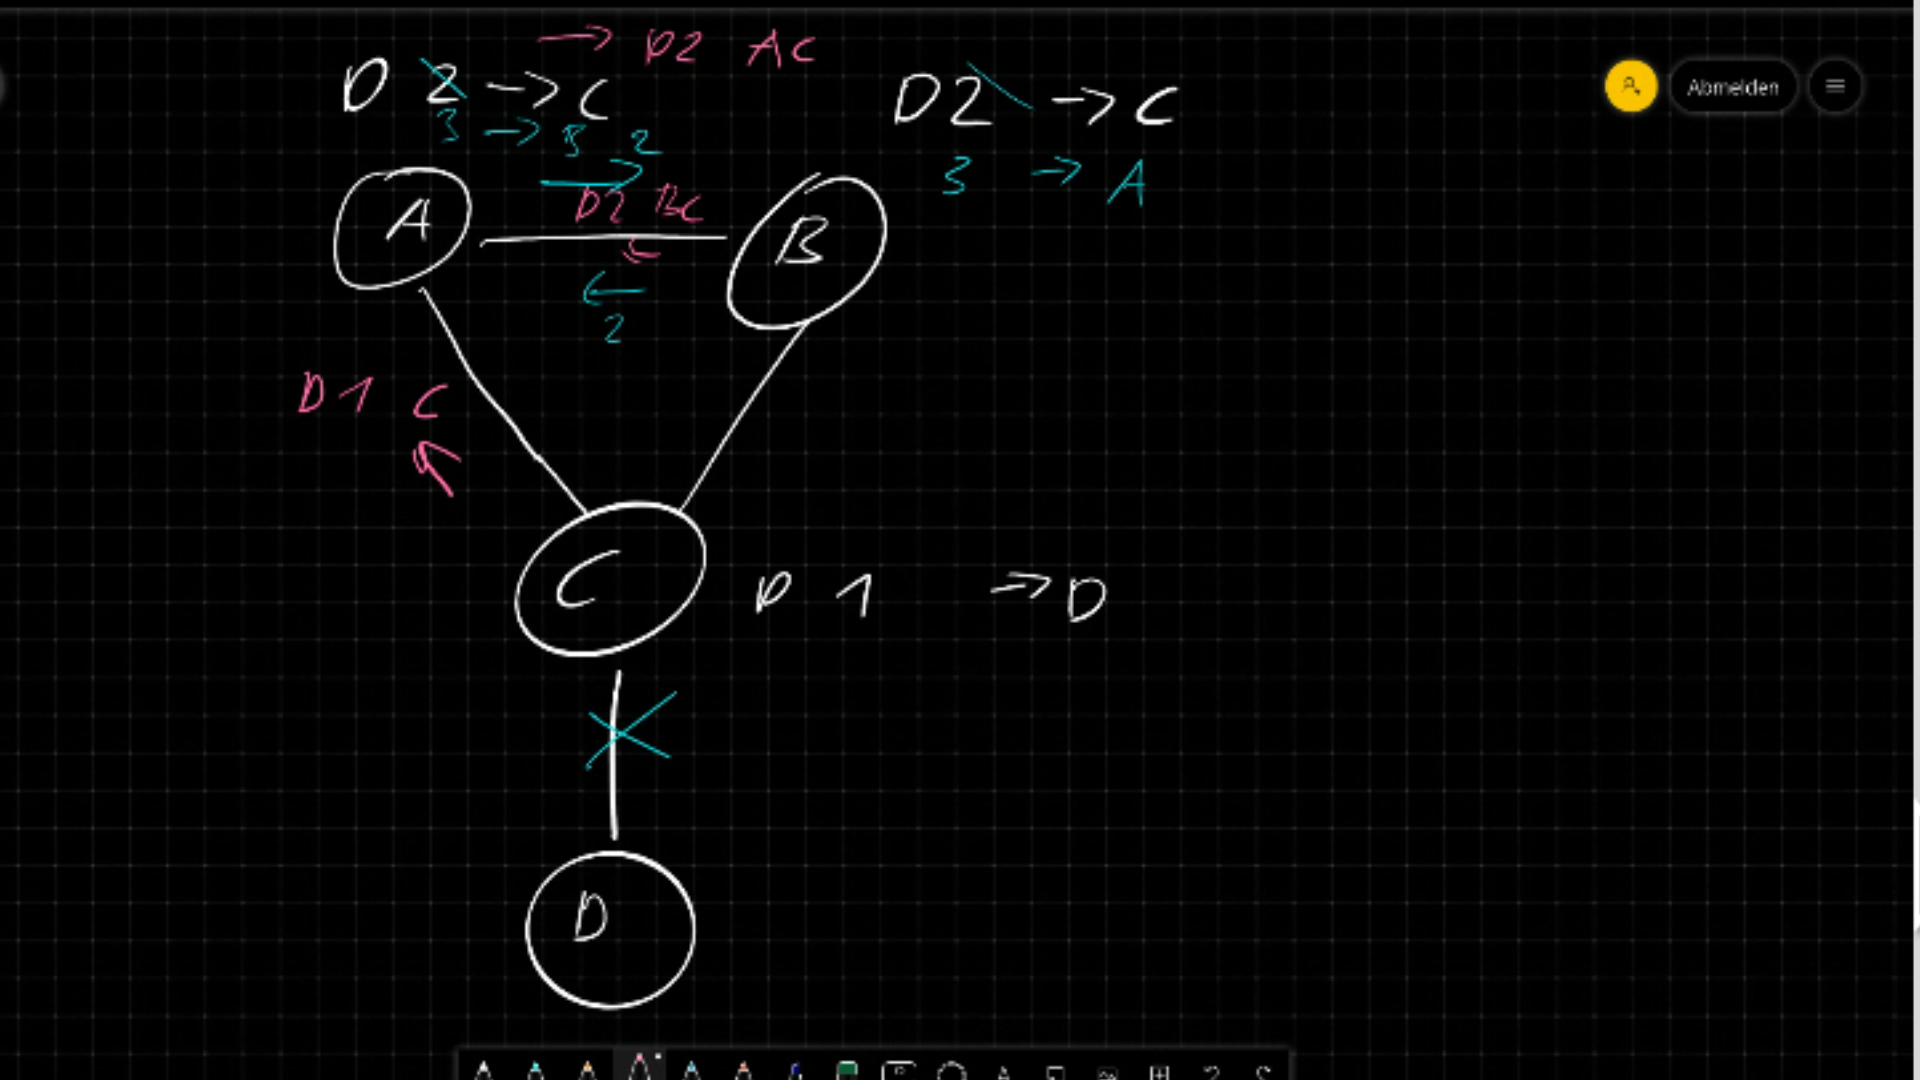
\includegraphics[width=\linewidth]{samplePVR} \\
	wird flächendeckend im Internet eingesetzt als Bordergateway Protokoll \\
	BGP \\
	Link-State-Routing \\
	Jeder Router hat ein komplettes Bild des Netztes \\
	Spanning Tree \\
	\subsection*{01.06.2021}
	spanning tree \\
	managed und unmanaged switch \\
	Ebene 1 Medienverbund \\
	Ebene 2 Frame-Verbund \\
	Ebene 3 Paketverbund \\
	Bridge Brücke zwischen Technologien z.B. Accesspoint \\
	Routing vs. Switching \\
	\subsection*{08.07.2021}
	Firewall Idee: Trennung zwischen unsicheren und sicheren Bereichen. \\
	Netzwerk Sicherheit: \\
	App-Gateway, Proxy, Paketfilter \\
	Permissive: was nicht verboten ist ist erlaubt
	Prohibitiv: was nicht erlaubt ist ist verboten. \\
	synpakte verbieten verhindert TCP Handshake \\
	Proxy prüft request auf Layer 7 \\
	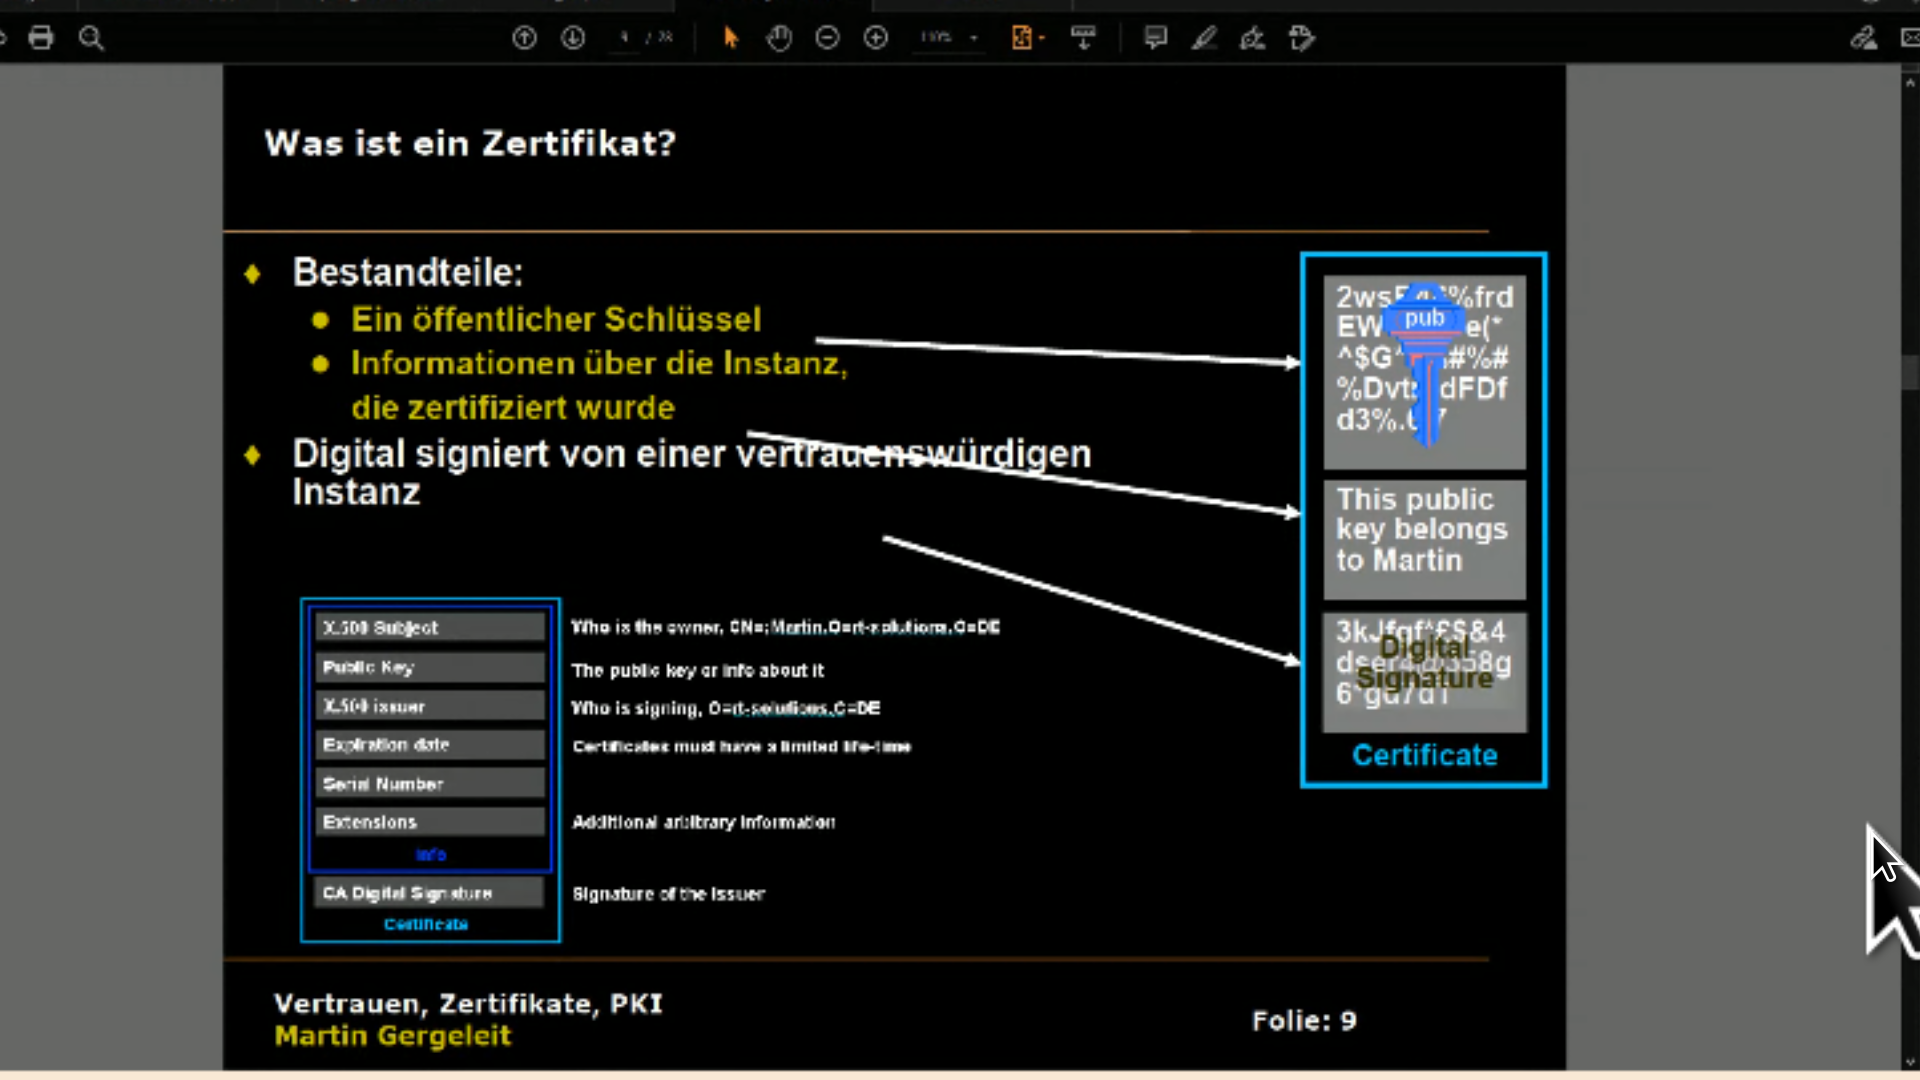
\includegraphics[width=\linewidth]{cert} \\
	Auth über certs \\
	Austellung eines Zertifikats \\
	In der Regel über RA mit Priv und Pubkey \\
	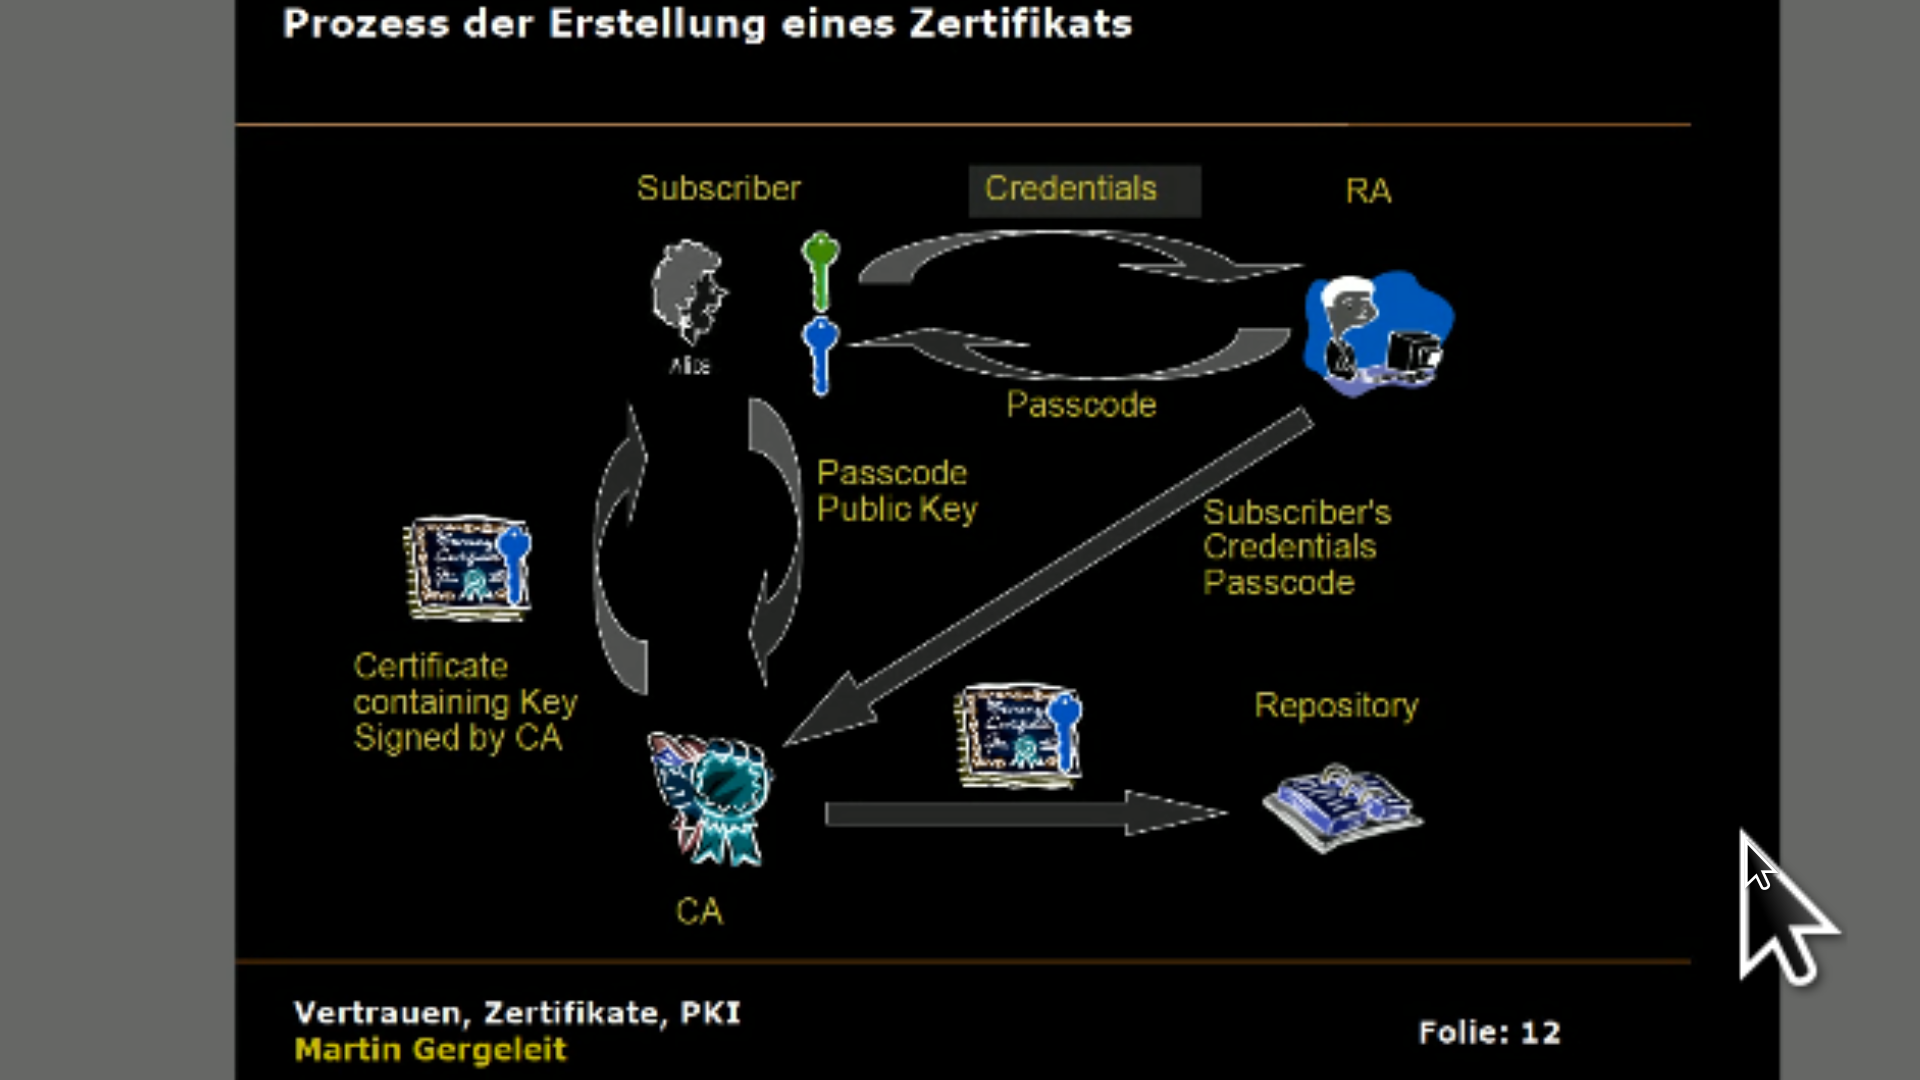
\includegraphics[width=\linewidth]{cert2} \\
	\subsection*{22.06.2021}
	firewall kann auch komplexer sein. \\
	dmz \\
	application gateway z.b. webproxy \\
	mehrstufige dmz \\
	\subsection*{29.06.2021}
	IPV6 \\
	größerer Adressbereich \\
	Mehr Struktur \\
	Anycast \\
	Einfacher Header schnelles Routing
	IPv6 zwanzig jahre als v4 40 Jahre alt. \\
	128 Bit \\
	viermal so lang wie IPv4 \\
	IPv6 in CIDR \\
	linkedlocal, sidelocal, global \\
	Router advertisment \\
	
\end{document}